\WarningFilter{latex}{Text page 25 contains only floats}

\begin{figure*}[tb!]
    \centering
    \begin{subfigure}[b]{0.29\textwidth}
        \centering
        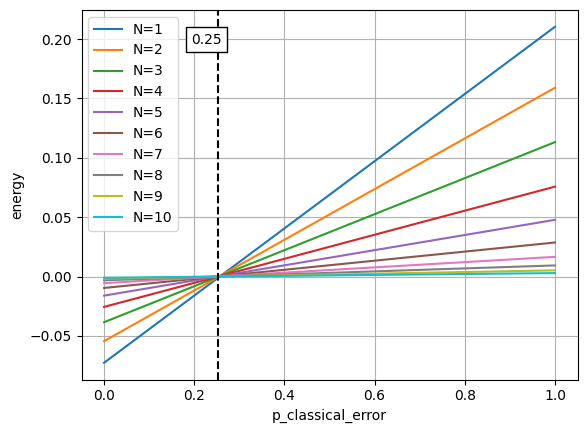
\includegraphics[width=\textwidth]{Appendix/plots/errors/numerical/Alice/Alice_energy_vs_p_class_comm_err.png}
        \caption{$H^{(1)}$}
    \end{subfigure}
    \hfill
    \begin{subfigure}[b]{0.29\textwidth}
        \centering
        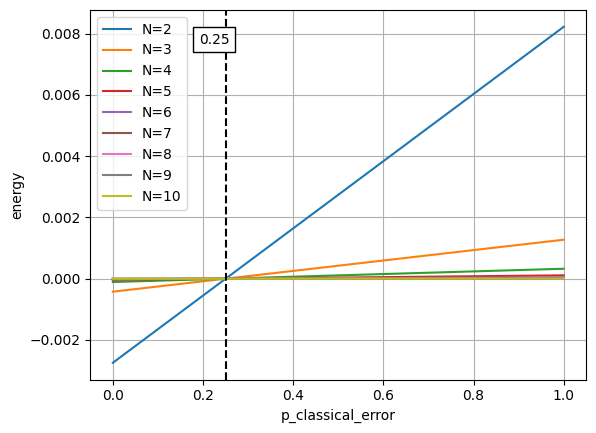
\includegraphics[width=\textwidth]{Appendix/plots/errors/numerical/NearestNeighbors/NN_X_energy_vs_p_class_comm_err.png}
        \caption{$H^{(2)}$, $\sigma_A = X_0$}
    \end{subfigure}
    \hfill
    \begin{subfigure}[b]{0.29\textwidth}
        \centering
        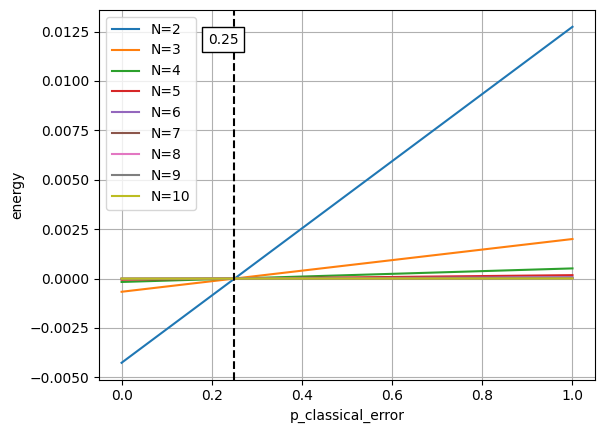
\includegraphics[width=\textwidth]{Appendix/plots/errors/numerical/NearestNeighbors/NN_Y_energy_vs_p_class_comm_err.png}
        \caption{$H^{(2)}$, $\sigma_A = Y_0$}
    \end{subfigure}

    \caption{Energy vs. Classical communication error for different \(N\) values. The linear degradation of the signal is evident across all models, with a consistent failure threshold where the expectation value crosses zero. The signal magnitude for the $H^{(2)}$ model visibly diminishes with increasing system size $N$.}
    \label{fig:energy_vs_classical_err_for_n}
\end{figure*}

\begin{figure*}[tb!]
    \centering
    \begin{subfigure}[b]{0.24\textwidth}
        \centering
        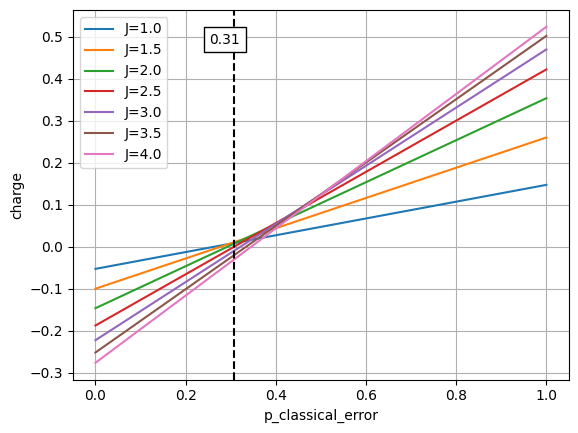
\includegraphics[width=\textwidth]{Appendix/plots/errors/numerical/Alice/N1/N1_charge_vs_p_classical_error.png}
        \caption{Charge, $N=1$}
    \end{subfigure}
    \hfill
    \begin{subfigure}[b]{0.24\textwidth}
        \centering
        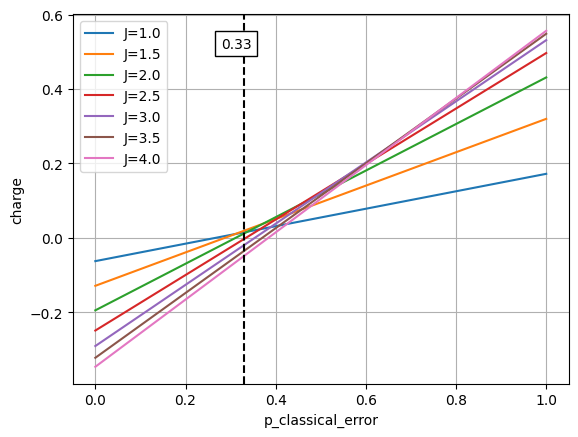
\includegraphics[width=\textwidth]{Appendix/plots/errors/numerical/Alice/N2/N2_charge_vs_p_classical_error.png}
        \caption{Charge, $N=2$}
    \end{subfigure}
    \hfill
    \begin{subfigure}[b]{0.24\textwidth}
        \centering
        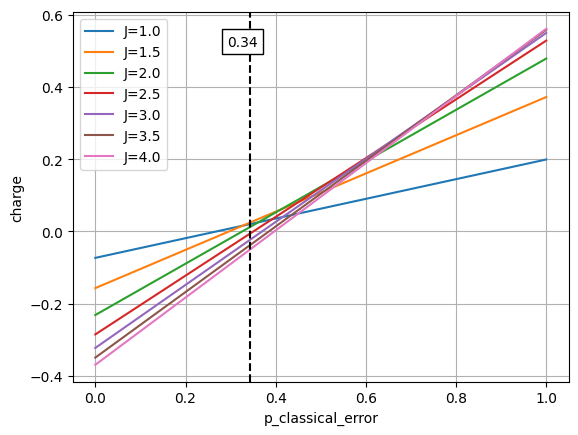
\includegraphics[width=\textwidth]{Appendix/plots/errors/numerical/Alice/N3/N3_charge_vs_p_classical_error.png}
        \caption{Charge, $N=3$}
    \end{subfigure}
    \hfill
    \begin{subfigure}[b]{0.24\textwidth}
        \centering
        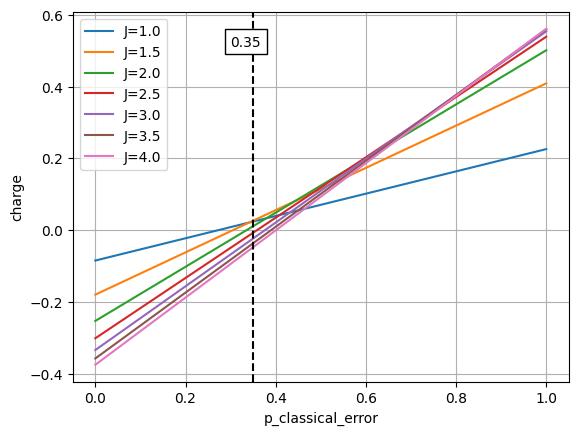
\includegraphics[width=\textwidth]{Appendix/plots/errors/numerical/Alice/N4/N4_charge_vs_p_classical_error.png}
        \caption{Charge, $N=4$}
    \end{subfigure}

    \vspace{0.5em}
    
    \begin{subfigure}[b]{0.24\textwidth}
        \centering
        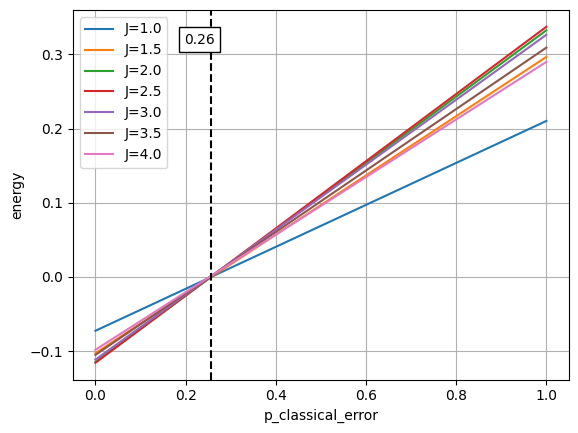
\includegraphics[width=\textwidth]{Appendix/plots/errors/numerical/Alice/N1/N1_energy_vs_p_classical_error.png}
        \caption{Energy, $N=1$}
    \end{subfigure}
    \hfill
    \begin{subfigure}[b]{0.24\textwidth}
        \centering
        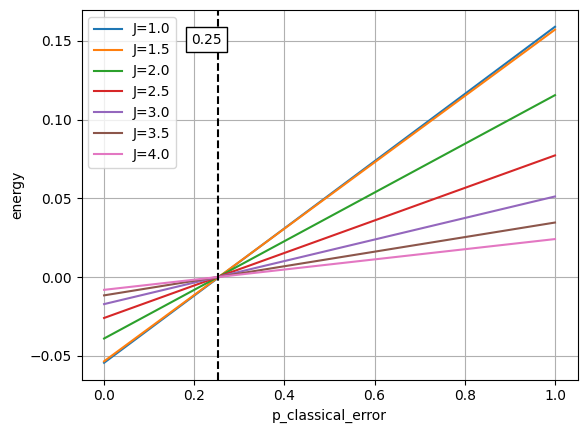
\includegraphics[width=\textwidth]{Appendix/plots/errors/numerical/Alice/N2/N2_energy_vs_p_classical_error.png}
        \caption{Energy, $N=2$}
    \end{subfigure}
    \hfill
    \begin{subfigure}[b]{0.24\textwidth}
        \centering
        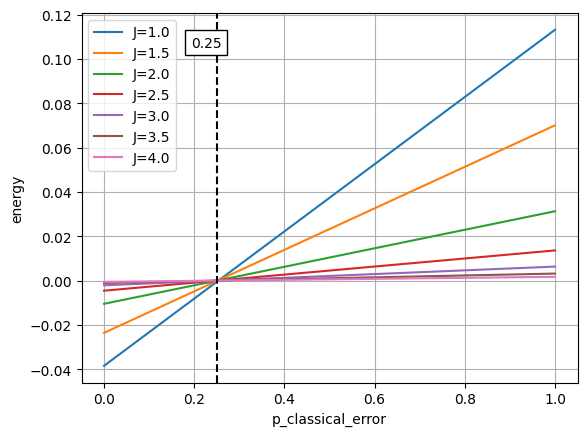
\includegraphics[width=\textwidth]{Appendix/plots/errors/numerical/Alice/N3/N3_energy_vs_p_classical_error.png}
        \caption{Energy, $N=3$}
    \end{subfigure}
    \hfill
    \begin{subfigure}[b]{0.24\textwidth}
        \centering
        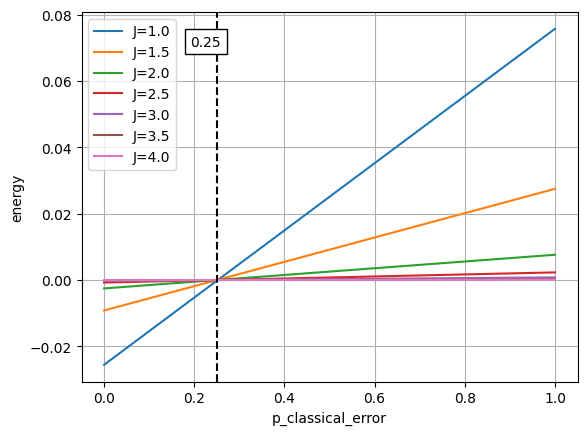
\includegraphics[width=\textwidth]{Appendix/plots/errors/numerical/Alice/N4/N4_energy_vs_p_classical_error.png}
        \caption{Energy, $N=4$}
    \end{subfigure}

    \caption{Classical communication error vs the coupling \(J\) for the star-interaction Hamiltonian $H^{(1)}$.}
    \label{fig:classical_err_alice_ham}
\end{figure*}

\begin{figure*}[tb!]
    \centering
    \begin{subfigure}[b]{0.29\textwidth}
        \centering
        
\includegraphics[width=\textwidth]{plots/errors/numerical/N2_charge_vs_p_classical_error.png}
        \caption{Charge, $N=2$}
    \end{subfigure}
    \hfill
    \begin{subfigure}[b]{0.29\textwidth}
        \centering
        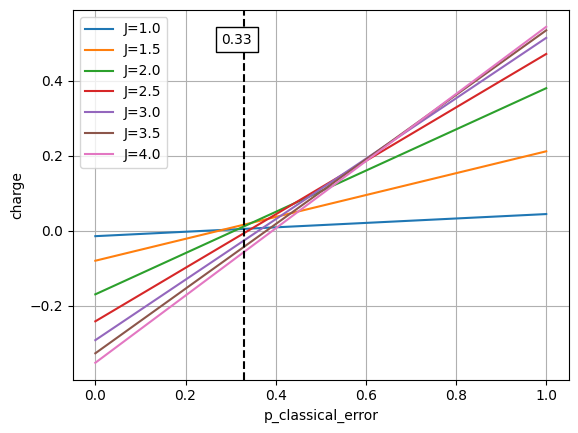
\includegraphics[width=\textwidth]{Appendix/plots/errors/numerical/NearestNeighbors/N3/X_N3_charge_vs_p_classical_error.png}
        \caption{Charge, $N=3$}
    \end{subfigure}
    \hfill
    \begin{subfigure}[b]{0.29\textwidth}
        \centering
        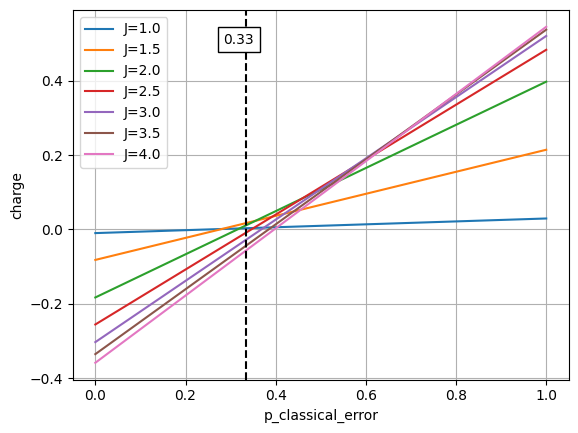
\includegraphics[width=\textwidth]{Appendix/plots/errors/numerical/NearestNeighbors/N4/X_N4_charge_vs_p_classical_error.png}
        \caption{Charge, $N=4$}
    \end{subfigure}

    \vspace{0.5em}
    
    \begin{subfigure}[b]{0.29\textwidth}
        \centering
        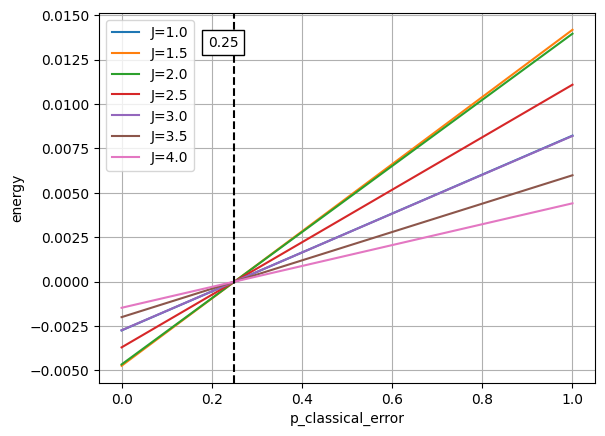
\includegraphics[width=\textwidth]{Appendix/plots/errors/numerical/NearestNeighbors/N2/X_N2_energy_vs_p_classical_error.png}
        \caption{Energy, $N=2$}
    \end{subfigure}
    \hfill
    \begin{subfigure}[b]{0.29\textwidth}
        \centering
        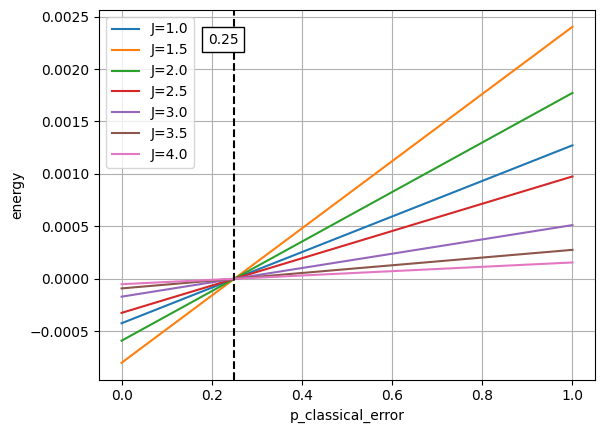
\includegraphics[width=\textwidth]{Appendix/plots/errors/numerical/NearestNeighbors/N3/X_N3_energy_vs_p_classical_error.png}
        \caption{Energy, $N=3$}
    \end{subfigure}
    \hfill
    \begin{subfigure}[b]{0.29\textwidth}
        \centering
        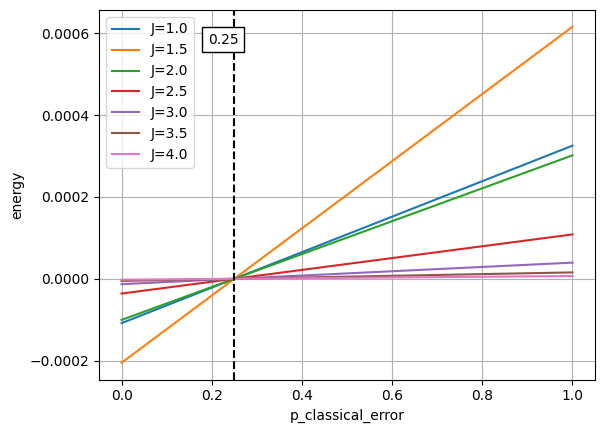
\includegraphics[width=\textwidth]{Appendix/plots/errors/numerical/NearestNeighbors/N4/X_N4_energy_vs_p_classical_error.png}
        \caption{Energy, $N=4$}
    \end{subfigure}

    \caption{Classical communication error vs the coupling \(J\) for the nearest-neighbor Hamiltonian $H^{(2)}$ with Alice Base \(\sigma_A = X_0\).}
    \label{fig:classical_err_nn_ham_x}
\end{figure*}

\begin{figure*}[tb!]
    \centering
    \begin{subfigure}[b]{0.29\textwidth}
        \centering
        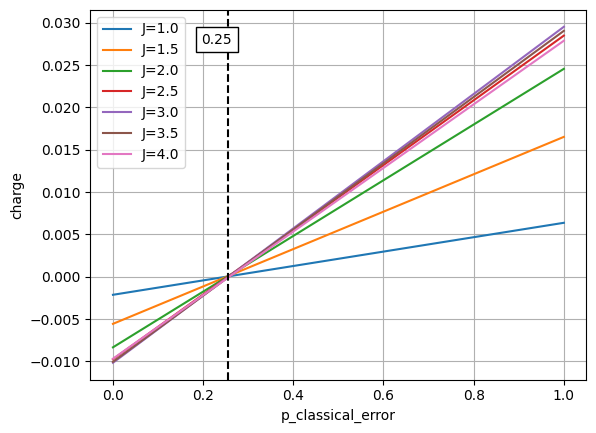
\includegraphics[width=\textwidth]{Appendix/plots/errors/numerical/NearestNeighbors/N2/Y_N2_charge_vs_p_classical_error.png}
        \caption{Charge, $N=2$}
    \end{subfigure}
    \hfill
    \begin{subfigure}[b]{0.29\textwidth}
        \centering
        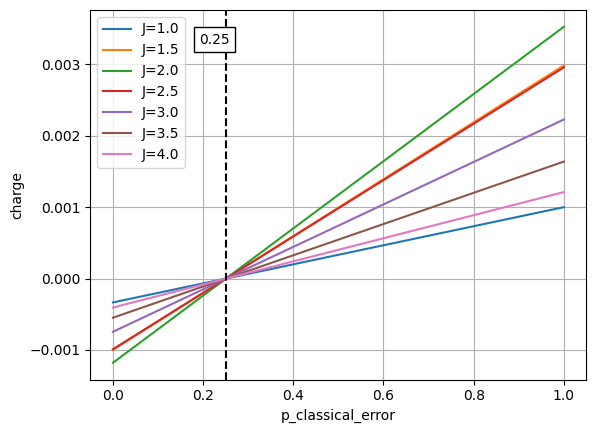
\includegraphics[width=\textwidth]{Appendix/plots/errors/numerical/NearestNeighbors/N3/Y_N3_charge_vs_p_classical_error.png}
        \caption{Charge, $N=3$}
    \end{subfigure}
    \hfill
    \begin{subfigure}[b]{0.29\textwidth}
        \centering
        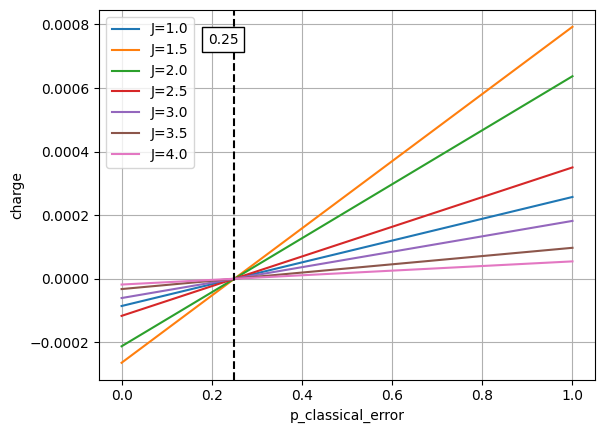
\includegraphics[width=\textwidth]{Appendix/plots/errors/numerical/NearestNeighbors/N4/Y_N4_charge_vs_p_classical_error.png}
        \caption{Charge, $N=4$}
    \end{subfigure}

    \vspace{0.5em}
    
    \begin{subfigure}[b]{0.29\textwidth}
        \centering
        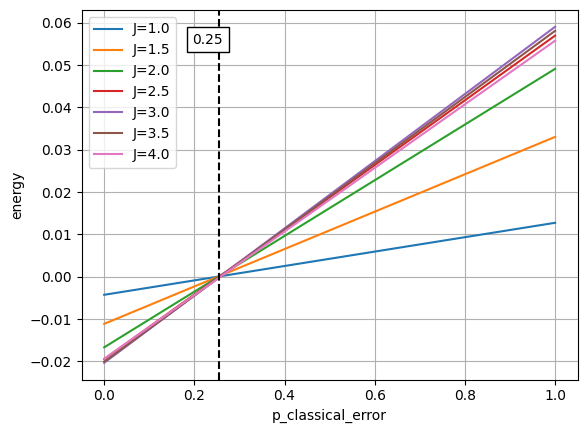
\includegraphics[width=\textwidth]{Appendix/plots/errors/numerical/NearestNeighbors/N2/Y_N2_energy_vs_p_classical_error.png}
        \caption{Energy, $N=2$}
    \end{subfigure}
    \hfill
    \begin{subfigure}[b]{0.29\textwidth}
        \centering
        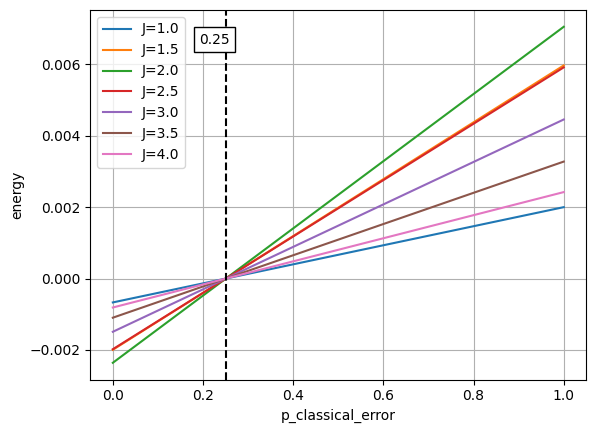
\includegraphics[width=\textwidth]{Appendix/plots/errors/numerical/NearestNeighbors/N3/Y_N3_energy_vs_p_classical_error.png}
        \caption{Energy, $N=3$}
    \end{subfigure}
    \hfill
    \begin{subfigure}[b]{0.29\textwidth}
        \centering
        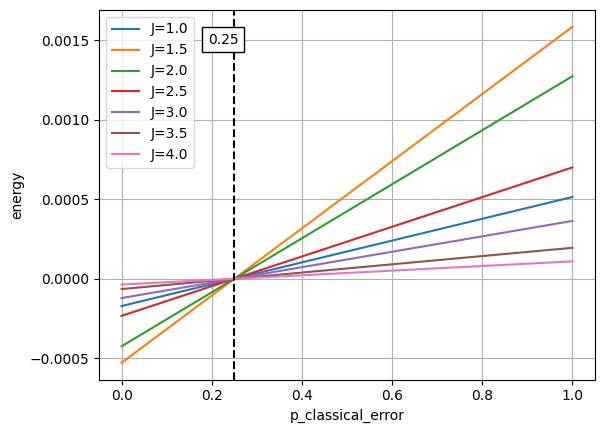
\includegraphics[width=\textwidth]{Appendix/plots/errors/numerical/NearestNeighbors/N4/Y_N4_energy_vs_p_classical_error.png}
        \caption{Energy, $N=4$}
    \end{subfigure}

    \caption{Classical communication error vs the coupling \(J\) for the nearest-neighbor Hamiltonian $H^{(2)}$ with Alice Base \(\sigma_A = Y_0\).}
    \label{fig:classical_err_nn_ham_y}
\end{figure*}

An error in the classical communication channel represents a scenario where the measurement outcome bit sent by Alice is flipped with a probability $p$ before it reaches Bob. This type of error directly impacts Bob's conditional operation, causing him to apply the incorrect unitary rotation. Consequently, the final state at Bob's side becomes a statistical mixture of the state corresponding to the intended outcome (transmitted with probability $1-p$) and the state corresponding to the flipped outcome (transmitted with probability $p$) \cite{QKDbyQET}. The resulting density matrix at Bob's site is given by:

\begin{equation*}
\begin{aligned}
\rho_{B,p} &= (1-p)\sum_{b}U_{B}(b)P_{A}(b)\rho_{gs}P_{A}(b)U_{B}^{\dagger}(b) \\
&+ p\sum_{b'=b\oplus1}U_{B}(b')P_{A}(b)\rho_{gs}P_{A}(b)U_{B}^{\dagger}(b')
\end{aligned}
\end{equation*}

This leads to a linear degradation of the expected signal, which can be expressed as \cite{QKDbyQET}:

\begin{equation*}
\langle\Delta O_{B}\rangle_{p} = (1-p)\langle\Delta O_{B}\rangle_{a=0} + p\langle\Delta O_{B}\rangle_{a=1}
\end{equation*}
